\hypertarget{probcut-standardabweichung-othello_pc_sigma.ipynb}{%
\section{Probcut Standardabweichung
(othello\_pc\_sigma.ipynb)}\label{probcut-standardabweichung-othello_pc_sigma.ipynb}}

\label{sec:pcsigma}

\begin{lstlisting}[language=Python]
%%HTML
<style>
.container { width:100% }
</style>
\end{lstlisting}

In diesem Notebook wird die für den Probcut Algorithmus benötigte
Standardabweichung in Abhängigkeit von der aktuellen Spielphase, welche
durch die Anzahl der Steine auf dem Spielfeld angegeben wird, bestimmt.
Dazu wird in verschiedenen Spielzuständen, jeweils eine Suche der Tiefe
\(d\) und eine Suche der Tiefe \(d'\) durchgeführt, und die Ergebnisse
als Datenpunkte gesammelt. Im Anschluss wird für jede Spielphase die
Varianz bestimmt, und diese mit einer geschlossenen Formel angenähert.

Das Notebook basiert auf der Implementation der Künstlichen Intelligenz,
welche daher im Folgenden eingebunden wird.

\begin{lstlisting}[language=Python]
%run othello_ai.ipynb
\end{lstlisting}

Für die statistische Betrachtung werden mehrere externe Bibliotheken
verwendet. Dazu gehören \passthrough{\lstinline!pandas!} und
\passthrough{\lstinline!csv!} für das Schreiben und Laden von
CSV-Dateien, \passthrough{\lstinline!sklearn!} für die Lineare
Regression, sowie \passthrough{\lstinline!matplotlib!} und
\passthrough{\lstinline!seaborn!} für die grafische Darstellung.

\begin{lstlisting}[language=Python]
import csv
import os
import pandas
import numpy as np
import sklearn.metrics as skl
import sklearn.linear_model as lm
import sklearn.preprocessing as pp
import matplotlib.pyplot as plt
import seaborn as sns
import math
\end{lstlisting}

\hypertarget{sammeln-von-datenpunkten}{%
\subsection{Sammeln von Datenpunkten}\label{sammeln-von-datenpunkten}}

Im der Funktion \passthrough{\lstinline!sample\_probcut\_values!} werden
zunächst einige Datenpunkte zur Bestimmung der Standardabweichung
gesammelt, indem in vielen verschiedenen Spielzuständen jeweils eine
tiefe und eine flache Suche durchgeführt wird. Die jeweiligen Tiefen
werden dabei durch die Parameter
\passthrough{\lstinline!shallow\_depth!} und
\passthrough{\lstinline!deep\_depth!} spezifiziert. Die verwendeten
Spielzustände werden ausgehen vom Startzustand durch zufälliges Ziehen
erreicht, welches in der KI Strategie
\passthrough{\lstinline!random\_ai!} implementiert wird. Es werden
insgesamt \passthrough{\lstinline!num\_games!} Spiele auf diese Weise
gespielt, und jeder Zustand entsprechend untersucht. Die so erhaltenen
Daten werden in einer CSV-Datei gespeichert.

\begin{lstlisting}[language=Python]
def sample_probcut_values(num_games, shallow_depth, deep_depth):
    fname = f'probcut_dataset_{PROBCUT_SHALLOW_DEPTH}_{PROBCUT_DEEP_DEPTH}.csv'
    file_exists = os.path.isfile(fname)
    if file_exists:
        print('using existing dataset')
    else:
        with open(fname, 'w', newline='') as file:
            writer = csv.writer(file, delimiter=',')
            writer.writerow(('moves', 'shallow', 'deep'))
            for i in range(num_games):
                state = GameState()
                while not state.game_over:
                    state = ai_make_move(random_ai, state, 0, None)
                    shallow_value = alphabeta(
                        state, PROBCUT_SHALLOW_DEPTH,
                        combined_heuristic, -math.inf, math.inf
                    )
                    deep_value = alphabeta(
                        state, PROBCUT_DEEP_DEPTH,
                        combined_heuristic, -math.inf, math.inf
                    )
                    print(f'shallow: {shallow_value}, deep: {deep_value}')
                    writer.writerow(
                        (state.num_pieces, shallow_value, deep_value))
            file.close()
\end{lstlisting}

Hier wird die Funktion \passthrough{\lstinline!sample\_probcut\_values!}
für die in der Probcut Implementierung verwendeten Suchtiefen
ausgeführt.

\begin{lstlisting}[language=Python]
sample_probcut_values(100, PROBCUT_SHALLOW_DEPTH, PROBCUT_DEEP_DEPTH)
\end{lstlisting}

Der Folgende Codeabschnitt lädt die zu verwendeten Datenpunkte aus einer
CSV-Datei. Dabei wird die externe Bibliothek
\passthrough{\lstinline!pandas!} zum Datenimport genutzt.

\begin{lstlisting}[language=Python]
filename = f'probcut_dataset_{PROBCUT_SHALLOW_DEPTH}_{PROBCUT_DEEP_DEPTH}.csv'
df = pandas.read_csv(filename)
shallow = np.array(df['shallow'])
deep = np.array(df['deep'])
moves = np.array(df['moves'])
\end{lstlisting}

Der folgende Code setzt die Ergebnisse der tiefen Suchen zu denen der
flachen Suchen in Form eines Scatterplots ins Verhältnis. Das
resultierende Schaubild ist in \autoref{fig:probcut_all_depths} zu
sehen.

\begin{lstlisting}[language=Python]
model = lm.LinearRegression()
model.fit(shallow.reshape(len(shallow), 1), deep)
plt.figure(figsize=(15, 10))
sns.set(style='whitegrid')
plt.scatter(shallow, deep)
plt.axvline(x=0.0, c='k')
plt.axhline(y=0.0, c='k')
plt.plot(shallow, shallow * model.coef_ + model.intercept_)
plt.xlabel('shallow search')
plt.ylabel('deep search')
plt.title('Probcut Values')
plt.show()
\end{lstlisting}

\begin{figure}[h]
    \centering
    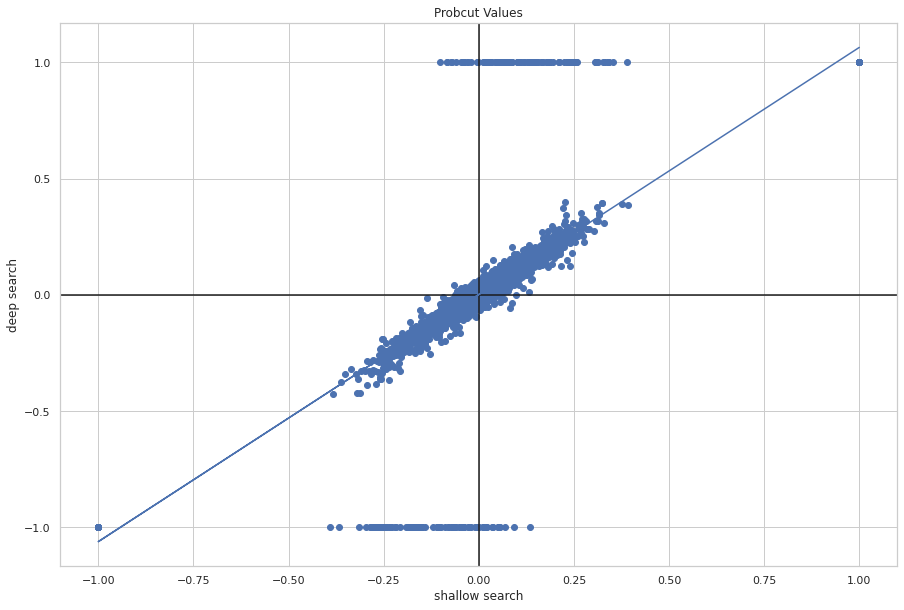
\includegraphics[width=\textwidth]{probcut_all_depths}
    \caption{Probcut Datenpunkte}
    \label{fig:probcut_all_depths}
\end{figure}

Wie zu erwarten, ist eine klare lineare Abhängigkeit zu erkennen, welche
durch die ebenfalls dargestellte Regressionsgerade hervorgehoben wird.
Die Ausreißer bei Deep Depth Werten von \(1\) und \(-1\) entstehen
dadurch, dass in diesen Spielzuständen, mit einer Tiefen Suche bereits
der Ausgang des Spiels bestimmt werden kann, während bei der Flachen
Suche noch die Heuristik verwendet wird. Theoretisch kann bereits hier
die Standardabeweichung ermittelt, und dann in Probcut genutzt werden.
Bei zusätzlicher Betrachtung der Anzahl von Steinen auf dem Spielfeld
stellt sich jedoch heraus, dass die Standardabweichung stark davon
abhängt. Durch Einbeziehung der Steinzahl bei der Ermittleung der
Standardabweichung lässt sich also eine genauere Aussage über die
Standardabweichung machen.

Der folgende Code berechnet die Standardabweichung pro Anzahl Steine auf
dem Spielfeld. Dazu werden zunächst für jede Anzahl an Steinen aus den
Daten die passenden Werte extrahiert. Für diese Teilmengen wird jeweils
die Varianz mit \passthrough{\lstinline!numpy!} berechnet. Die
Standardabweichung ist dann die positive Wurzel aus der Varianz. Die
Anzahl an Steinen und die dazugehörige Standardabweichung werden in den
Feldern \passthrough{\lstinline!x!} und \passthrough{\lstinline!y!}
gespeichert.

\begin{lstlisting}[language=Python]
x = np.empty(0)
y = np.empty(0)

for i in range(5, 64):
    shallow_c = shallow[moves == i]
    deep_c = deep[moves == i]
    variance = np.var(np.stack([shallow_c, deep_c], axis=1))
    x = np.append(x, i)
    y = np.append(y, math.sqrt(variance))
\end{lstlisting}

Im Anschluss werden diese Daten visualisiert, um zu beurteilen, wie die
Standardabweichung durch eine geschlossene Formel angenähert werden
kann. Der Scatterplot kann in \autoref{fig:probcut_sigma_by_disccount}
betrachtet werden.

\begin{lstlisting}[language=Python]
plt.figure(figsize=(15, 10))
sns.set(style='whitegrid')
plt.scatter(x, y)
plt.axhline(y=0.0, c='k')
plt.xlabel('number of disks on the board')
plt.ylabel('standard deviation')
plt.title('Standard Deviation')
plt.show()
\end{lstlisting}

\begin{figure}[h]
    \centering
    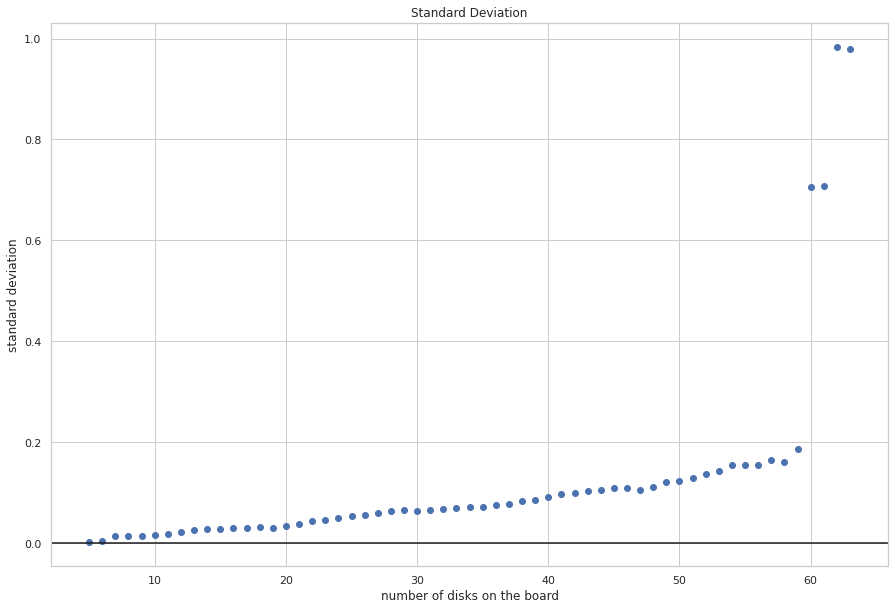
\includegraphics[width=\textwidth]{probcut_sigma_by_disccount}
    \caption{Probcut Standardabweichung abhängig von der Steinzahl}
    \label{fig:probcut_sigma_by_disccount}
\end{figure}

Bei der Betrachtung ergibt sich, dass im Bereich zwischen 5 und 58 Zügen
eine annähernd quadratische Abhängigkeit vorliegt. Daher wird dieser
Bereich mittels Polynomieller Regression angehähert und visualisiert

Folgender Code berechnet das Regressionspolynom zweiten Gerades der
Standardabweichung in Abhängigkeit von der Anzahl der Steine auf dem
Spielfeld mit \passthrough{\lstinline!sklearn!} und stellt dieses, wie
in \autoref{fig:probcut_sigma_polynomial_regression} zu sehen, grafisch
dar.

\begin{lstlisting}[language=Python]
indices = np.argwhere(x <= 58)
xnew = x[indices]
ynew = y[indices][:,0]
polynomial_features= pp.PolynomialFeatures(degree=2)
xpoly = polynomial_features.fit_transform(xnew)

model = lm.LinearRegression()
model.fit(xpoly, ynew)

theta0 = model.intercept_
theta1, theta2, theta3 = model.coef_
a = np.arange(0.0, 60.0, 0.01)
b = theta0 + (theta1 + theta2) * a + theta3 * a**2

plt.figure(figsize=(15, 10))
sns.set(style='whitegrid')
plt.scatter(xnew, ynew)
plt.axhline(y=0.0, c='k')
plt.plot(a, b)
plt.xlabel('number of disks on the board')
plt.ylabel('standard deviation')
plt.title('Standard Deviation')
plt.show()
\end{lstlisting}

\begin{figure}[h]
    \centering
    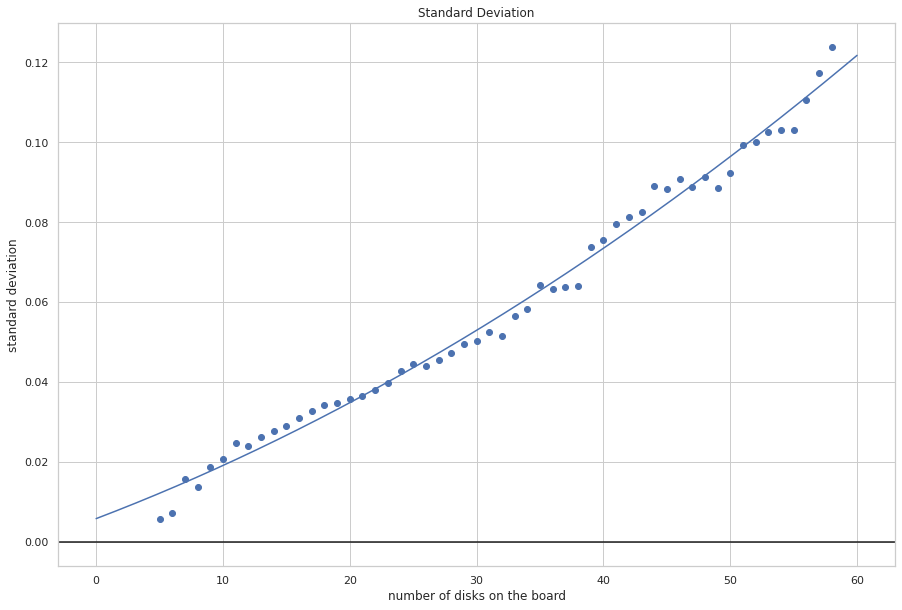
\includegraphics[width=\textwidth]{probcut_sigma_polynomial_regression}
    \caption{Annäherung der Standardabweichung durch Polynomielle Regression}
    \label{fig:probcut_sigma_polynomial_regression}
\end{figure}

Hier wird das Regressionspolynom ausgegeben, welches näherungsweise die
Standardabweichung in Abhängigkeit von der Anzahl an Spielsteinen auf
dem Spielfeld berechnet

\begin{lstlisting}[language=Python]
print(theta0, '+', theta1 + theta2, '* x +', theta3, '* x**2')
\end{lstlisting}

Die hier ausgegebenen Funktion wird in der Probcut Implementierung zur
Bestimmung der Standardabweichung genutzt.
